\documentclass[10pt,a4paper]{article}
\usepackage[utf8]{inputenc}
\usepackage[italian]{babel}
\usepackage{amsmath}
\usepackage{amsfonts}
\usepackage{amssymb}
\usepackage{graphicx}
\usepackage[left=2cm,right=2cm,top=2cm,bottom=2cm]{geometry}
\newcommand{\rem}[1]{[\emph{#1}]}

\author{Gruppo AC \\ Federico Belliardo, Giulia Franchi, Francesco Mazzoncini}
\title{Esercitazione N.8: Oscillatore sinusoidale a ponte di Wien con OpAmp.}
\begin{document}
\maketitle
\section{Scopo dell'esperienza}
Lo scopo dell'esperienza è realizzare un oscillatore ad onda sinusoidale a ponte di Wien utilizzando un OpAmp modello TL081.\\
\section{Montaggio del circuito e misura del loop gain}
Abbiamo montato il circuito in fig. \ref{oscillatore} utilizzando $R_1=9.95\pm0.08\,k\Omega$, $R_2=9.81\pm0.08\,k\Omega$, $R_3=9.82\pm0.08\,k\Omega$, $R_4=9.89\pm0.08\,k\Omega$, $R_5=9.88\pm0.08\,k\Omega$, un potenziometro con $P_{MAX}=10.47\pm0.09\,k\Omega$, due condensatori $C_1=9.9\pm0.4\,nF$ e $C_2=9.9\pm0.4\,nF$. Le tensioni di alimentazione sono $V_{+} = 15.09 \pm 0.08 \, V$ e $V_{-} = -15.08 \pm 0.08 \, V$.\\

\begin{figure}[!htb]
  \centering
  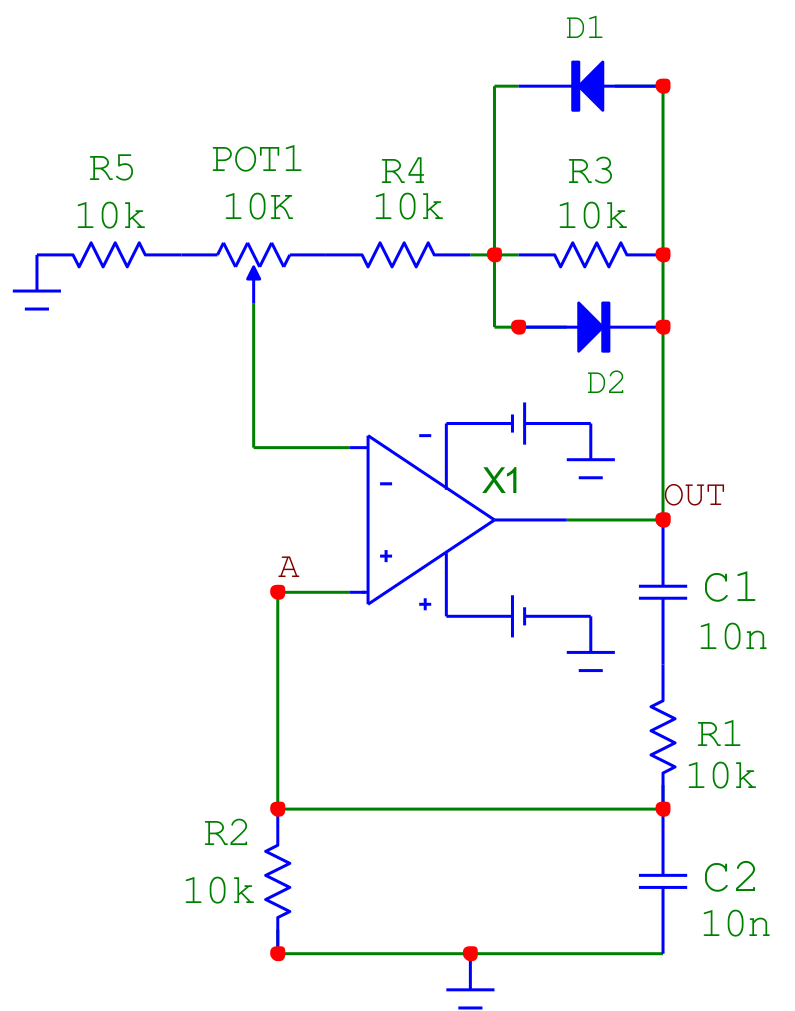
\includegraphics[scale=0.25]{ponteDiWien.png}
\caption{Circuito oscillatore a ponte di Wien.}
\label{oscillatore}
\end{figure}

Si attendono quindi per i due sottocircuiti $R_1 C_1$ e $R_2 C_2$ le frequenze di taglio $f_1=\frac{1}{2 \pi R_1C_1} = 1.62 \pm 0.07 \, kHz $ e $f_2=\frac{1}{2 \pi R_2C_2} = 1.62 \pm 0.07 \, kHz$.\\

Abbiamo scollegato il punto A dall'ingresso non invertente dell'OpAmp, inviando al suo posto attraverso il generatore di funzioni un segnale sinusoidale di ampiezza pari a circa $250\,mV$ (in realtà $V_{+} = 252 \pm 2 \, mV$) con frequenza tra $500\,Hz$ e $3\,kHz$ \footnote{Da notare il fatto che l'intervallo considerato comprende anche la frequenza di taglio $f_1 \sim f_2$.}, in uscita osserviamo un segnale oscillate.\\
In tab. \ref{tabella} abbiamo riportato i valori di $V_+$, $V_A$, del loro sfasamento $\phi$ e del loro rapporto $\beta A_V$.\\

\begin{table}[!htb]
\centering
\begin{tabular}{|c|c|c|c|c|c|c|c|}
\hline
$f\,(Hz)$ & $ \sigma f \, (Hz)$ & $V_A \, (V)$ & $\sigma V_A \, (V)$ & $\vert \beta A_V \vert$ & $\sigma \vert \beta A_V \vert$ & $ \phi \, ( \pi \, rad)$ & $ \sigma \phi \, ( \pi \, rad)$\\
\hline
507 & 5 & 0.118 & 0.001 & 0.468 & 0.005 & 0.231 & 0.005\\
708 & 7 & 0.140 & 0.001 & 0.556 & 0.006 & 0.159 & 0.006\\
902 & 9 & 0.152 & 0.001 & 0.603 & 0.006 & 0.112 & 0.007\\
1260 & 10 & 0.164 & 0.002 & 0.651 & 0.009 & 0.040 & 0.003\\
1570 & 20 & 0.164 & 0.002 & 0.651 & 0.009 & 0.000 & 0.003\\
1900 & 20 & 0.164 & 0.002 & 0.651 & 0.009 & -0.049 & 0.002\\
2550 & 30 & 0.156 & 0.001 & 0.619 & 0.006 & -0.110 & 0.002\\
3100 & 30 & 0.150 & 0.001 & 0.595 & 0.006 & -0.156 & 0.003\\
\hline
\end{tabular}
\label{tabella}
\caption{Misure del loop-gain dell'oscillatore in funzione della frequenza.}
\end{table}

In seguito abbiamo riportato il diagramma di Bode dell'attenuazione e dello sfasamento in fig.\ref{bode} e fig.\ref{sfasamento} rispettivamente.\\


\begin{figure}[!htb]
  \centering
  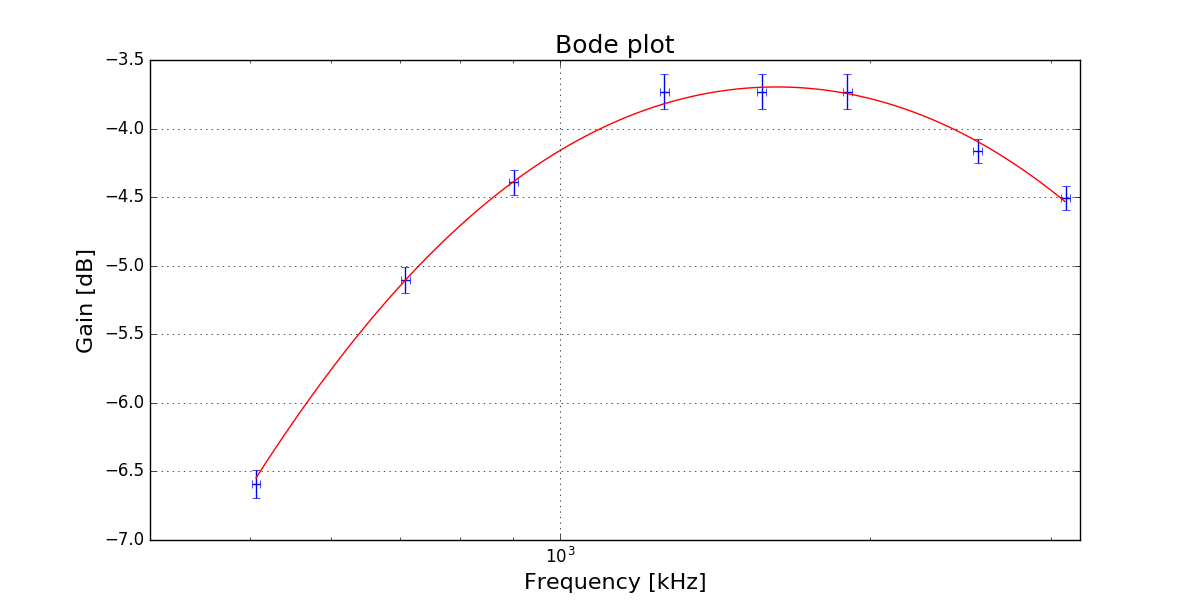
\includegraphics[scale=.5]{bode.png}
\caption{Diagramma di bode del ponte di Wien.}
\label{bode}
\end{figure}


\begin{figure}[!htb]
  \centering
  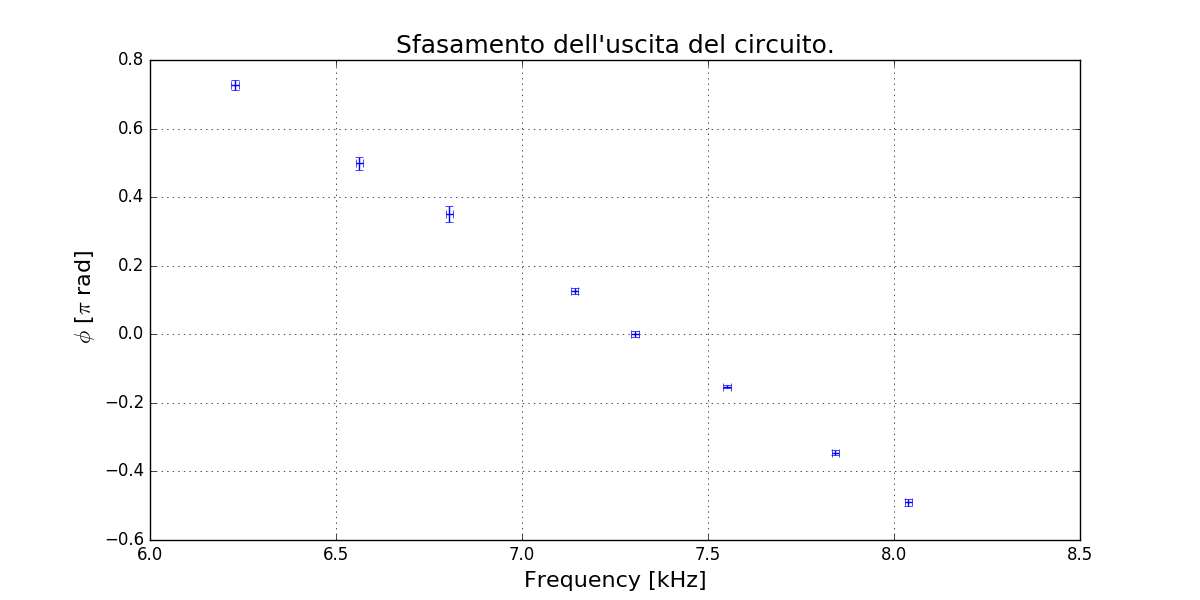
\includegraphics[scale=.5]{sfasamento.png}
\caption{Sfasamento del ponte di Wien.}
\label{sfasamento}
\end{figure}

Per il fit di $\vert \beta A_V \vert$ si è utilizzata la funzione \emph{curvefit} della libreria \emph{pylab} con l'opzione \emph{$absolute\,sigma = "true"$}, poichè abbiamo considerato gli errori come statistici. Riportiamo di seguito parametri $A_{max}$ e $f_0$ della funzione $ \vert \beta A_V \vert = \frac{A_{max} f_0 f}{\sqrt{(f^2-f_0^2)^2+9 f_0^2 * f^2}}$, con la relativa matrice di covarianza: $A_{max} = 1.964 \pm 0.005$, $f_0 = 1620 \pm 20 \, Hz$,  $ \Sigma_{ij} = \left( \begin{array}{cc}
2.38 \cdot 10^{+2} & 2.00 \cdot 10^{-2} \\ 
2.00 \cdot 10^{-2} & 2.56 \cdot 10^{-2}\\
\end{array} \right)$. Con un $\chi^2/ndof = 1.47/5$.\\


Per il fit dello sfasamento \footnote{Eseguito su una scala logaritmica nelle ascisse.} riportiamo di seguito parametri $a$ e $b$ della retta $y=ax+b$, con la relativa matrice di covarianza: $a = -0.490 \pm 0.008$, $b = 1.56\pm 0.03$,  $ \Sigma_{ij} = \left( \begin{array}{cc}
6.84 \cdot 10^{-5} & -2.18 \cdot 10^{-4} \\ 
-2.18 \cdot 10^{-4} & 6.99 \cdot 10^{-4}\\
\end{array} \right)$. Con un $\chi^2/ndof = 3/5$.\\

Da questo fit si ottiene che lo sfasamento è nullo per $f_0 = 1.5 \pm 0.2 , kHz$ \footnote{L'errore è grande poichè avendo eseguito il fit con le ascisse logaritmiche abbiamo dovuto esponenziare il rapporto tra i coefficienti forniti da \emph{curve fit} per ottenere la frequenza critica.}.\\

Riportiamo di seguito i tre valori ottenuti per la frequenza di taglio del circuito, con i relativi metodi utilizzati:\\

\begin{itemize}
\item Misura diretta dello zero dello sfasamento: $f_0 = 1570 \pm 20 \, Hz$.
\item Fit di $\vert \beta A_V \vert$: $f_0 = 1620 \pm 20 \, Hz$.
\item Fit dello sfasamento: $f_0 = 1.5 \pm 0.2 , kHz$
\end{itemize}

Le ultime due misure sono confrontabili con la frequenza di taglio dei sottocircuiti RC entro l'errore. La misura diretta è affetta da sottostima dell'errore perchè non abbiamo considerato l'intervallo di frequenze in cui lo sfasamento poteva essere ritenuto nullo, l'ampiezza di questo intervallo avremmo dovuto considerarla nell'errore della misura.\\

Il valore di $A_{max}$ non risulta essere tre (e quindi $\vert \beta A_V \vert$ non risulta essere uno per la frequenza di taglio) poichè le misure sono state prese con il potenziometro in una posizione generica. Si vede dal grafico fig. \ref{bode} che la massima amplificazione si ha per la frequenza di taglio.\\

L'amplificazione massima del segnale è $A_max = 1 - \frac{R_{feedback}}{R_{verso massa}}$, osserviamo che aumentando la frazione del potenziometro che partecipa alla resistenza di feedback aumenta l'ampiezza dell'uscita.\\

\section{Comportamento del circuito al variare del potenziometro}
Abbiamo sconnesso il generatore di funzioni e riconnesso il punto A all'ingresso non-invertente dell'OpAmp e abbiamo osservato il segnale in uscita al variare della resistenza del potenziometro. Si nota che se abbassiamo la resistenza di \emph{feedback} fino a $R_{f} = 3.11 \pm 0.03 \, k\Omega$ il segnale oscillante scompare e l'uscita va a zero, poichè per $A_V < 3$, cioè $\beta A_V < 1$ (sotto la condizione di Barkhausen) il segnale rientrando varie volte nel circuito viene attenuato fino a scomparire ( $(\beta A_V)^n \rightarrow 0$ per $n \rightarrow \infty$) . Mentre aumentando la resistenza di feedback aumenta l'ampiezza del segnale in uscita, perde la forma sinuosidale finchè si raggiunge clipping a $13.4\,V$, come si vede in fig. \ref{clipping}.

\begin{figure}[!htb]
  \centering
  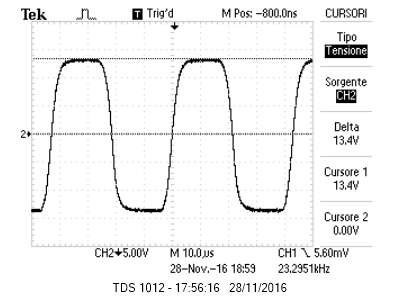
\includegraphics[scale=.5]{clipping.png}
\caption{Clipping ad alta amplificazione dell'oscillatore.}
\label{clipping}
\end{figure}

Il segnale è perfettamente sinusoidale solamente per la posizione del potenziometro a cui comincia l'oscillazione (condizione di Barkhausen verificata) al di sopra di questo valore è satabile in ampiezza (grazie ai diodi) ma distorta come si vede nella figura \ref{distorta}.\\

\begin{figure}[!htb]
  \centering
  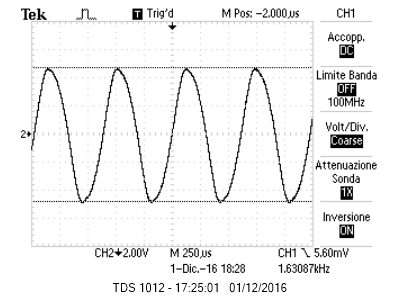
\includegraphics[scale=.5]{ondaDistorta.png}
\caption{Distorsione dell'onda fuori dalla condizione di Barkhausen.}
\label{distorta}
\end{figure}

\section{Misura della frequenza di oscillazione}
Riportiamo la frequenza di oscillazione ottenuta dal frequenzimetro dell'oscilloscopio: $f_0 = 1.64 \pm 0.01 \, kHz$. Ruotando il potenziometro (senza arrivare al clipping) la frequenza non cambia, così come non cambia al variare dell'alimentazione \footnote{Comunque superiore in modulo a $11\,V$ come prescritto dal manuale dell'opAmp.}. Quando si verifica clipping il frequenzimeto dell'oscillografo segna una variazione di frequenza.\\

\section{Misura del guadagno $A_v$ open loop}
Abbiamo impostato il potenziometro (ruotando la vite) in modo da raggiungere il punto di innesco dell’oscillazione e si è disconnesso il circuito di retroazione dall’ingresso non invertente, sostituendolo con un segnale sinusoidale di ampiezza $V_+=0.992 \pm 0.008\,V$ emesso dal generatore di funzioni. Si è misurato $V_{OUT} = 3.00 \pm 0.02 \,V$, da questi otteniamo: $A_V = 3.02 \pm 0.03$.\\

Alla frequenza per cui lo sfasamento della rete RC è nullo l'amplificazione vale $\beta = \frac{1}{3}$, dunque ci aspettiamo (condizione di Barkhausen) $A_V = 3$ per la posizione del potenziometro per cui iniziano a verificarsi le oscillazioni. Sottolineo che siste una sola posizione del potenziometro per cui si ha $A_V = 3$. Come spiegato nella sezione successiva i diodi permettono di controllare l'ampiezza del segnale in uscita anche se non è verificata la condizine di Barkhausen, cioè anche se $\beta A_V > 1$ il segnale non diverge (\emph{clipping}) rientrando nel sistema varie volte ma rimane ad un valore finito.

\section{Rimozione dei diodi}
I diodi hanno la funzione di entrare in conduzione quando la corrente che attraversa la resistenza $R_3$ diventa grande (dunque quando è alta la tensione $V_OUT$). Se succede ciò la corrente passa attraverso i diodi (con bassa resistenza) dunque diminuisce la resistenza di feedback e di conseguenza l'amplificazine e l'ampiezza del segnale $V_{OUT}$, finchè i diodi non tornano in interdizione. Questo permette di avere oscillazioni stabili per varie posizioni del potenziometro anche se non sono oscillazioi sinusoidali.\\
Se togliamo i diodi si osserva clipping (opAmp in saturazione) per tutte le posizoni del potenziometro, superato il valore del potenziometro a cui $A_V = 3$, $\beta A_V$ diventa maggiore di 1 e il segnale passando più volte nel circuito porta l'opAmp in saturazione, $(\beta A_V)^n \rightarrow \ininity$ per $n \rightarrow \infty$.\\

\end{document}